\documentclass[12pt,titlepage]{article}
\usepackage[table]{xcolor}
\usepackage{longtable}
\usepackage[utf8]{inputenc}
%Language of Document Elements like Figure or Table
\usepackage[english]{babel}
\usepackage[bookmarks]{hyperref}
\usepackage{pdfpages}
\usepackage{graphicx}
\usepackage{float}
\usepackage{array}
\usepackage[justification=centering]{caption}
\usepackage{enumitem}
\usepackage{chngcntr}
\usepackage{lscape}
\usepackage{fancyhdr}
\usepackage{listings}
\usepackage{hyperref}
\usepackage{nameref}
\usepackage{tabularx}
\usepackage[a4paper,width=160mm,top=25mm,bottom=25mm]{geometry}

%Syntax-highlighting]
%\usepackage{minted}
%\usemintedstyle{vs}

%Each Section in a new Page
\let\oldsection\section
\renewcommand\section{\clearpage\oldsection}

%Set space around and between lists
\setlist[enumerate]{noitemsep, topsep=0cm}
\setlist[itemize]{noitemsep, topsep=0cm}

%Figure/Table Numbering style "Section Number.figure counter
\renewcommand{\thefigure}{\arabic{section}.\arabic{figure}}
\renewcommand{\thetable}{\arabic{section}.\arabic{table}}

%Reset figure/table counter after section change
\counterwithin{figure}{section}
\counterwithin{table}{section}

\hypersetup{
	colorlinks,
	linkcolor={black},
	citecolor={black},
	urlcolor={black}
}

\colorlet{punct}{red!60!black}
\definecolor{background}{HTML}{EEEEEE}
\definecolor{delim}{RGB}{20,105,176}
\colorlet{numb}{magenta!60!black}

\newcommand{\todonl}[1]{\newline\textcolor{red}{TODO: #1}\PackageWarning{TODO:}{#1!}}
\newcommand{\todo}[1]{\textcolor{red}{TODO: #1}\PackageWarning{TODO:}{#1!}}

%Set Paragraph indent to null
\setlength{\parindent}{0pt}
% Smaler Table Space
\renewcommand{\arraystretch}{1.5}

% renamig of section to Abschnitt \autoref 
\addto\extrasenglish{%
	\def\sectionautorefname{Abschnitt}%
}

% renamig of subsubsection to Abschnitt \autoref 
\addto\extrasenglish{%
	\def\subsubsectionautorefname{Abschnitt}%
}

% renamig of subsection to Abschnitt \autoref 
\addto\extrasenglish{%
	\def\subsectionautorefname{Abschnitt}%
}
%rename Figure zu Abbildung
\addto\captionsenglish{\renewcommand{\figurename}{Abbildung}}

%rename Tabe zu Tabelle
\addto\captionsenglish{\renewcommand{\tablename}{Tabelle}}

\title{Software-Defined Netzwerk im Campus Bereich}
\author{Sandro Kaspar, Philipp Albrecht, Jessica Kalberer}
\date{28.02.2017}

\pagestyle{fancy}
\lhead{Software-Defined Netzwerk im Campus Bereich}
\begin{document}
\pagenumbering{Roman} 



\includepdf{pdfincludes/titlepage}

\newpage
%new Title for tableofcontent
\renewcommand{\contentsname}{Inhaltsverzeichnis}
\tableofcontents
\newpage
\pagenumbering{arabic}

\section{Abstract}
Der Abstract richtet sich an den Spezialisten auf dem entsprechenden Gebiet und 
beschreibt daher in erster Linie die (neuen, eigenen) Ergebnisse und Resultate der 
Arbeit. Es umfasst nie mehr als eine Seite, typisch sogar nur etwa 200 Worte (etwa 
20 Zeilen). Es sind keine Bilder zu verwenden.

\subsection{Version 2}

Ziel dieser Studienarbeit war die Evaluation des Cisco Digital Network Architecture (DNA) Center, der Software Defined Access Lösung von Cisco, für die Führungsunterstützungsbasis der Schweizer Armee. Der erste Schwerpunkt lag dabei auf der Installation des DNA Centers und der Konfiguration sowie Integration eines Campus Netzwerkes. Für das DNS-, DHCP- und IP-Adress-Management (IPAM) wird im Campus Netzwerk Infoblox eingesetzt. Für die Benutzerverwaltung sowie Zugriffskontrolle wird die Cisco Identity Services Engine (ISE) verwendet.

Nach dem Einrichten des Campus Netzwerkes lag der zweite Schwerpunkt auf der Definition von Benutzer- und Geräteprofilen, um den einzelnen Mitarbeitern der Schweizer Armee den Netzwerkzugriff zu ermöglichen und die Zugriffsrechte der einzelnen Mitarbeiter oder eines Teams zentral zu regeln. Des Weiteren sollte mit DNA Assurance eine proaktive Überwachung, Fehlerbehebung und Optimierung des Netzwerkes sichergestellt werden. Mit diesen Informationen sollten wöchentliche Reports über den Status des Netzwerks per E-Mail oder Slack Message versendet werden.\\
\\
Die Inbetriebnahme des Campus Netzwerkes gestaltete sich schwieriger als erwartet. Viele der Schritte sind nur teilweise automatisiert und es ist sehr viel manueller Aufwand nötig. Als Beispiel kann hier die LAN Automation aufgeführt werden. Mit Hilfe dieser sollten sich Netzwerkgeräte automatisiert via PnP in Betrieb nehmen und konfigurieren lassen. Dieser Prozess ist allerdings sehr fehleranfällig und funktioniert nur unzuverlässig, sodass die Inbetriebnahme des Underlay Netzwerkes erst nach mehreren Versuchen korrekt ausgeführt werden konnte. 
Des Weiteren funktionieren viele Funktionen des DNA Centers nur mit spezifischen Versionen von ISE und IOS-XE. Dies führte zu weiteren Komplikationen, da dies vom Hersteller so nicht dokumentiert ist. 
Durch diese Komplikationen wurde der ganze Provisionierungsprozess verzögert. 
\\
Abschliessend kann gesagt werden, das für die Installation und Konfiguration des DNA Centers mehrere Tage, wenn nicht Wochen eingerechnet werden müssen. Zudem muss im optimalen Fall ein Green Field vorliegen, da zur Zeit kein bestehendes Netzwerk ohne Unterbrüche migriert werden kann. Bei der Installation sollten die empfohlenen Softwareversionen genauestens eingehalten werden, da sonst die volle Funktionalität des DNA Centers nicht gewährleistet werden kann. Beim Kauf des DNA Centers ist es am einfachsten, gleich auch einen Experten von Cisco aufzubieten, um diese Appliance komplett in der gewünschten Umgebung in Betrieb zu nehmen. 

%\subsection{Ausgangslage}

%\subsection{Ziele der Arbeit}
%Das grundsätzliche Ziel ist eine Evaluation des Cisco Software Defined Networking. Im ersten Schritt beinhaltet das die %Inbetriebnahme und Konfiguration von den folgenden Komponenten:
%\begin{itemize}
%	\item Cisco DNA Center Appliance
%	\item Integration Infoblox (One Platform Solution für DNS, DHCP, IPAM)
%	\item Integration Cisco ISE (Access and Authentification Control)
%	\item Integration Campus Labor Netzwerk
%\end{itemize}
%Im zweiten Schritt sollen UseCases durchgespielt werden, die den folgenden Umfang abdecken:
%\begin{itemize}
%	\item Definierung von Benutzer- und Geräteprofile, um basierend auf Geschäftsanforderungen die Zugriffsrechte und Netzwerksegmentierung zu verwalten und so das Netzwerk sicher zu halten.
%	\item DNA Analytics and Assurance für eine proaktive Überwachung, Fehlerbehebung und Optimierung des Netzwerks.
%	\item IP Address Management Tool im DNA Center.
%	\item Wöchentliche Reports über Campus Netzwerk-Status via E-Mail oder Slack
%\end{itemize}

%\subsection{Ergebnisse}



\newpage
\appendix
\pagenumbering{Roman}

% !TeX encoding = UTF-8
\section{Sitzungsprotokolle}

\subsection{Sitzungsprotokoll 27.02.2018}

\paragraph{Sitzungsteilnehmer}
\begin{itemize}	
	\item Laurent Metzger 
	\item Philipp Albrecht
	\item Sandro Kaspar
	\item Jessica Kalberer
\end{itemize}

\paragraph{Traktanden}
\begin{itemize}	
	\item Projektstart
	\item Besprechung genaue Aufgabenstellung und nächste Schritte
\end{itemize}

\paragraph{Beschlüsse (Diskussion)}
\begin{itemize}	
	\item Evaluieren eines Software Defined Network im Campus Bereich für FUB.
	\item Anleitung für FUB für die Erstellung eines SD Networks mittels DNA Center.
	\item Freie Hand bei Gestaltung wöchentlicher Reports, da nicht alle Möglichkeiten bekannt.
	\item Geräte werden erst Mitte März 2018 geliefert
	\item Offene Frage: Vorgaben auf welcher Plattform Projekt laufen soll (Dropbox, gitHub)?
\end{itemize}

\paragraph{Offene Punkte (erledigt vor nächster Sitzung)} \mbox{}
\begin{table}[H]
	\rowcolors{2}{gray!25}{white}
	\centering
	\begin{tabularx}{\textwidth}{X | p{4.5cm}}
		\rowcolor{gray!50}
		\textbf{Was} & \textbf{Verantwortlichkeit} \\
		\hline	
		Projektplan mit Meilensteinen erstellen	& Philipp \\	
		Sitzungsprotokoll vom 27.02.2018 erstellen & Jessica \\
		Beschreibung der SD-A Lösung mit Vorteilen im Vergleich zu klassischem Campus Design (Management Summary) &	Sandro \\
		Module 2 Lesson 2 auf Cisco Learning Library anschauen (Part 1 und Part 2) & Philipp, Sandro, Jessica \\
		Dokumentation vorbereiten (Latex) anhand Strukturierungsbeispiel 2 & Jessica \\
		Zeiterfassung Tool vorbereiten & Jessica \\	
	\end{tabularx}
	\label{tab:my-label}
\end{table}

\paragraph{Nächster Termin}
\begin{itemize}	
	\item Meeting mit Betreuer: 06. März 2018, 10 Uhr, 60 Minuten
	\item Meeting mit Industriepartner: 08. März 2017, 14 Uhr, 120 Minuten
\end{itemize}

\paragraph{Kommende Abwesenheiten} \mbox{}\\
keine

\newpage





\subsection{Sitzungsprotokoll 06.03.2018}

\paragraph{Sitzungsteilnehmer}
\begin{itemize}	
	\item Laurent Metzger 
	\item Urs Baumann 
	\item Philipp Albrecht
	\item Sandro Kaspar
	\item Jessica Kalberer
\end{itemize}

\paragraph{Traktanden}
\begin{itemize}	
	\item Aufgabenstellung schriftlich vom Betreuer erhalten? Bekommen wir diese noch?
	\begin{itemize}
		\item erhalten wir in den letzten zwei Wochen
	\end{itemize}
	\item Zeiterfassung mit Toggl / Waffle.io / GitHub Issues so sinnvoll oder anders gewünscht?
	\begin{itemize}
		\item Tools passen, jedoch den Betreuern noch Zugang zu allen Tools geben
	\end{itemize} 
	\item Business Dresscode für Besprechung mit Industriepartner gewünscht?
	\begin{itemize}
		\item Nein, normale anständige Kleidung reicht
	\end{itemize}
	\item Teilnehmer Besprechung Industriepartner und deren Rollen?
	\begin{itemize}
		\item FUB Leiter vom Netzwerk mit einem Mitarbeiter
	\end{itemize}
	\item Was muss für die Besprechung mit dem Industriepartner vorbereitet werden?
	\begin{itemize}
		\item wir werden in erster Linie Informationen von FUB erhalten
		\item Grafik vorbereiten um eine Übersicht über unsere Tools zu zeigen
	\end{itemize}
	\item Arbeit auf GitHub private oder public? Waffle.io wenn private 5 Dollar / Monat
	\begin{itemize}
		\item Industriepartner am Donnerstag nochmals darauf ansprechen
	\end{itemize}
	\item Technologien einzeln genauer beschreiben notwendig?
	\begin{itemize}
		\item Technologien im technischen Bericht genauer beschreiben (SDA, DNA,..)
	\end{itemize}
\end{itemize}

\paragraph{Beschlüsse (Diskussion)}
\begin{itemize}	
	\item Use Cases Bereiche (ca. 10 Use Cases generieren). Unterscheidung welche Änderung das DNA Center bringt. Welche Use Cases sind neu? Use Cases müssen anfangs nicht komplett ins Detail beschrieben werden. Vielleicht zuerst User Stories generieren und daraus dann die Use Cases ableiten. Diese können dann mit Industriepartner abgeglichen werden, ob diese mit ihm übereinstimmen. Beispiele:
	\begin{itemize}
		\item Definierung von Benutzer- und Geräteprofile, um basierend auf Geschäftsanforderungen die Zugriffsrechte und Netzwerksegmentierung zu verwalten und so das Netzwerk sicher zu halten
		\item Durch APIs, Erstellung von wöchentlichen Reports per E-Mail
	\end{itemize}
	\item GitHub private oder public?
	\begin{itemize}
		\item Wird mit Industriepartner am nächsten Donnerstag direkt abgeklärt, aber wahrscheinlich ist es egal das wir es public machen
		\item Zugriffe für GitHub, Toggl, Waffle.io für Betreuer einrichten
	\end{itemize} 
	\item Technologien welche für unsere Arbeit essentiell sind im technischen Bericht festhalten, wie beispielsweise DNA Center, VXLAN, LISP. Doch Technologien wie BGP müssen nicht weiter dokumentiert werden, da genügend Cisco Quellen verfügbar sind und bekannt sein sollte.
	\item Projektmanagement gewünschter Inhalt:
	\begin{itemize}
		\item Projektplan
		\item Arbeitspakete
		\item Risikomanagement
		\item Testprotokoll (um Use Cases zu überprüfen)
	\end{itemize}
	\item Sitzung am Donnerstag mit Industriepartner für uns erst um 15:30 Uhr
	\begin{itemize}
		\item Dresscode für Meeting normal wie immer
		\item Präsentation mit Industriepartner Dresscode edel erwünscht mit Hemd etc.
	\end{itemize}
	\item Netzwerk-Umgebung: es muss noch eine passende Netzwerk-Topologie erstellt werden
	\begin{itemize}
		\item Hardware
		\begin{itemize}
			\item 4 x Catalyst 9300
			\item 4 x Catalyst 3850
		\end{itemize}
		\item VMs werden von Betreuer erstellt und wir erhalten VPN Zugriff auf die Server, falls wir Hardware Zugriff benötigen, befinden sich die Switches im Netzwerklabor.
		\begin{itemize}
			\item ISE, Infobox (Betreuer)
			\item DHCP, DNS, NTP (Ubuntu VM)
		\end{itemize}
	\end{itemize}
	\item Traktanden jeweils am Montagabend vorher an Betreuer senden.
	\item Kosten des Projektes
	\begin{itemize}
		\item Hardware DNA Center um die 90'000 Fr, Switch je à 10'000 Fr. Grundsätzlich wird alles von Urs im Netzwerklabor installiert. Softwaretechnisch kann alles an Cisco retourniert werden, wenn etwas nicht mehr bootet
	\end{itemize}
\end{itemize}

\paragraph{Offene Punkte (erledigt vor nächster Sitzung)} \mbox{}
\begin{table}[H]
	\rowcolors{2}{gray!25}{white}
	\centering
	\begin{tabularx}{\textwidth}{X | p{4.5cm}}
		\rowcolor{gray!50}
		\textbf{Was} & \textbf{Verantwortlichkeit} \\
		\hline	

		Zugriffe auf GitHub, Waffle.io und Toggl an Betreuer senden & Sandro \\
		Grafik vorbereiten für Übersicht über unsere Tools & Philipp \\
		GitHub private oder public mit FUB abklären am Donnerstag & Philipp, Sandro, Jessica \\
		Eingesetzte Technologien dokumentieren & Jessica \\
		Netzwerk-Topologie Vorschlag & Philipp \\
		Risiko-Management Tabelle & Sandro \\
		Use Cases vorbereiten (ca. 10 Use Cases generieren) & Philipp, Sandro, Jessica \\
		Sitzungsprotokoll in Latex übernehmen & Jessica \\
		Sitzungsprotokoll Traktanden jeweils spätestens Montagabend an Betreuer	& Jessica \\
		Testprotokoll Vorlage erstellen anhand von Use Cases & Jessica \\

	\end{tabularx}
	\label{tab:my-label}
\end{table}

\paragraph{Nächster Termin}
\begin{itemize}	
	\item Sitzung mit Industriepartner: 08. März 2018, 15.30 Uhr, 30 Minuten
	\item Sitzung mit Betreuer: 13. März 2018, 15.10 Uhr, 60 Minuten
\end{itemize}

\paragraph{Kommende Abwesenheiten} \mbox{}\\
keine

\newpage






\subsection{Sitzungsprotokoll 08.03.2018}

\paragraph{Sitzungsteilnehmer}
\begin{itemize}	
	\item Laurent Metzger 
	\item Urs Baumann
	\item Laurent Billas FUB
	\item Serge Pidoux FUB
	\item Philipp Albrecht
	\item Sandro Kaspar
	\item Jessica Kalberer
\end{itemize}

\paragraph{Traktanden}
\begin{itemize}	
	\item Arbeit auf GitHub private oder public? Waffle.io wenn private 5 Dollar / Monat
	\item Vorstellung unserer internen Organisationsstruktur
	\item Wird SDA zur Zeit schon benutzt?
	\item Aktuelle Infrastruktur
	\begin{itemize}
		\item Anzahl Benutzer
		\item Anzahl Netzwerkgeräte
		\item Wie viele Personen betreuen zur Zeit diese Infrastuktur? 
	\end{itemize}
\end{itemize}

\paragraph{Beschlüsse (Diskussion)}
\begin{itemize}	
	\item Sicherheit ist der Mittelpunkt bei der FUB. Entsprechende Use Cases definieren:
	\begin{itemize}
		\item Benutzer- und Geräteprofile Definition ist ein sehr wichtiger Punkt für die FUB. Sie möchten gerne wissen wie diese Definition auf einem ISE aussehen 
		\item Use Case: Austausch eines Switches oder Netzwerk-Gerätes
		\item sicherstellen das wir die erhaltenen Use Case richtig verstanden haben und dies mit ihnen nochmals abklären, falls etwas nicht ganz klar oder unpräzise
		\item wir werden mind. 4 Use Cases von der FUB erhalten, welche Ihnen besonders wichtig sind. Spätestens bis ende März 2018.			
	\end{itemize}
	\item Netzwerk-Umgebung: es muss noch eine passende Netzwerk-Topologie erstellt werden
	\begin{itemize}
		\item Hardware
		\begin{itemize}
			\item 4 x Catalyst 9300
			\item 4 x Catalyst 3850
			\item 1 Cisco 3650CX - Büro-Switch (herausfinden wie diese Switche im DNAC integriert werden können)
			\item 2 ISR4431
		\end{itemize}
		\item VMs werden von Betreuer erstellt und wir erhalten VPN Zugriff auf die Server, falls wir Hardware Zugriff benötigen, befinden sich die Switches im Netzwerklabor.
		\begin{itemize}
			\item ISE, Infobox (Betreuer - Lizenzen erhalten wir von der FUB)
			\item DHCP, DNS, NTP (Diese Dienste sind nicht separat, sondern auf der Infobox vorhanden und können dort eingerichtet werden.
		\end{itemize}
	\end{itemize}
	\item DNA-Center inkl. Material sollte ca. in 1-2 Wochen gesendet werden.
	\item Dimensionen des aktuellen FUB Netzes:
	\begin{itemize}
		\item Ganzes Führungsnetz Schweiz mittels MPLS
		\item Anzahl User permanent ein paar Tausend, aber ist sehr variabel je nach Einsatz. Wichtiger Punkt der abzuklären gilt wäre, werden die maximal erlaubten Geräte überschritten? Wo liegen die Limiten?
		\item Kennenlernen der Tools und abklärung ob diese Technologien 
	\end{itemize}
	\item GitHub kann public genutzt werden, da Informationen von FUB schon vorher gefiltert.
	\item SDA wird noch nicht benutzt, wir sollen diese Technologien für die Evaluieren.
\end{itemize}

\paragraph{Offene Punkte (erledigt vor nächster Sitzung)} \mbox{}
\begin{table}[H]
	\rowcolors{2}{gray!25}{white}
	\centering
	\begin{tabularx}{\textwidth}{X | p{4.5cm}}
		\rowcolor{gray!50}
		\textbf{Was} & \textbf{Verantwortlichkeit} \\
		\hline	
		Netzwerktopologie mit zusätzlichen Geräten & Philipp \\	
		Risiko-Management Tabelle & Sandro \\
		Sitzungsprotokoll Traktanden spätestens Montagabend an Betreuer	& Jessica \\		
	\end{tabularx}
	\label{tab:my-label}
\end{table}

\paragraph{Nächster Termin}
\begin{itemize}	
	\item Meeting mit Betreuer: 13. März 2018, 15.10 Uhr, 60 Minuten
\end{itemize}

\paragraph{Kommende Abwesenheiten} \mbox{}\\
keine

\newpage






\subsection{Sitzungsprotokoll 13.03.2018}

\paragraph{Sitzungsteilnehmer}
\begin{itemize}	
	\item Laurent Metzger 
	\item Urs Baumann
	\item Philipp Albrecht
	\item Sandro Kaspar
	\item Jessica Kalberer
\end{itemize}

\paragraph{Traktanden}
\begin{itemize}	
	\item Genauigkeit der Dokumentation der Technologien
	\item Wie ist es mit Quellen umzugehen?
	\item Netzwerktopologie besprechen
\end{itemize}

\paragraph{Beschlüsse (Diskussion)}
\begin{itemize}	
	\item Netzwerktopologie
	\begin{itemize}
		\item Core Layer kommt darauf an welche Modelle wir bekommen, um dies genauer spezifizieren zu können
		\begin{itemize}
			\item 9300-24T-A (Lizenz: Cisco DNA Advantage für 3 Jahre) ohne Uplinks
			\item Die genauen Modelle werden uns von Herrn Metzger noch bekannt gegeben		
		\end{itemize}
		\item Green: Out of Bound Management
		\item 3650CX kann selbst kein VXLAN und muss an 9300 angeschlossen werden
		\item Unterschiedliche Gebäude in Netzwerktopologie erwähnen
		\item 9300 zwischen Border und Control Node
		\item zwischen den Switchen L3 Routing Protokolle
		\item mit L2 auf Server zugriff vom 9300 Distribution Core her
		
		\item 9300 Unterschied der einzelnen Modelle mehr nur Perfomance
		\item Anmerkung: 3850XS nicht der beste Router in Core in einer Produktiven Umgebung
		
		\item 3850 aktuell bei FUB in Verwendung
		\item 9300 sind neu geplant
	\end{itemize}
	\item Wireless = Out of Scope, sollte unbedingt in der Dokumentation erwähnt und als optional definiert werden.
	\item DNAC Konfiguration von Switches (theoretisch ein Use Case)
	\begin{itemize}
		\item Bleibt die Verbindung bestehen bei Änderungen?
		\item Port Konfigurationen werden nicht kontrolliert
		\item Route Policies werden fix überschrieben
	\end{itemize}
	\item Netzwerktopologie wird von Herrn Metzger noch FUB gezeigt (informell)
	\item Verkabelungsplan erstellen: da keine Uplinks vorhanden, werden wahrscheinlich Port 1-4 für das verwendet
	\item Regelmässige Updates per Mail mit Dokumentation an Betreuer
	\item Quellen HSR intern keine Vorgaben, so wie angefangen weiterführen
\end{itemize}

\newpage 

\paragraph{Offene Punkte (erledigt vor nächster Sitzung)} \mbox{}

\begin{table}[H]
	\rowcolors{2}{gray!25}{white}
	\centering
	\begin{tabularx}{\textwidth}{X | p{4.5cm}}
		\rowcolor{gray!50}
		\textbf{Was} & \textbf{Verantwortlichkeit} \\
		\hline
		Genaue Modelle der Switche bekanntgeben & Laurent Metzger \\	
		Verkabelungsplan erstellen (Switch Ports) & Sandro \\
		IP-Adressen Plan & Philipp, Sandro, Jessica \\
		Mapping zwischen SDA und LISP Name Definitions & Jessica \\
		Regelmässige Updates der Doku an Betreuer & Philipp, Sandro, Jessica \\
	\end{tabularx}
	\label{tab:my-label}
\end{table}

\paragraph{Nächster Termin}
\begin{itemize}	
	\item Meeting mit Betreuer: 20. März 2018, 15.10 Uhr, 60 Minuten
\end{itemize}

\paragraph{Kommende Abwesenheiten} \mbox{}\\
keine
\newpage





\subsection{Sitzungsprotokoll 20.03.2018}

\paragraph{Sitzungsteilnehmer}
\begin{itemize}	
	\item Laurent Metzger 
	\item Urs Baumann
	\item Philipp Albrecht
	\item Sandro Kaspar
	\item Jessica Kalberer
\end{itemize}

\paragraph{Traktanden}
\begin{itemize}	
	\item Use Cases Industriepartner
	\item Verkabelungsplan
	\item LabNetzwerkArchitektur
	\item Zwischenstand aktuelle Dokumentation
	\item Dokumentatorisches: Quellenangaben
	\item Genaue Modelle der Switche (Laurent Metzger) - kommt noch
	\item IP Adress Plan - Vorgabe von Lab Infrastruktur (Urs Baumann) - kommt noch
	\item IPv6 Unterstützung? (Out of Scope - es werden private IPv4 Adressen verwendet RFC1918)
\end{itemize}

\paragraph{Beschlüsse (Diskussion)}
\begin{itemize}	
	\item Use Cases werden bis 27.März 2018 vom Industriepartner übergeben (Herr Metzger wird nochmal bei FUB nachhaken, damit diese wirklich geliefert werden)
	\item Netzwerk Architektur wurde nach Besprechung mit FUB noch angepasst. Es werden zwei weitere Router im Core Layer hinzugefügt und die Catalyst 3850 in den Distribution Layer hoch geschoben
	\item Im Core Layer wird für den Cisco ISR 4431 ein Modul hinzugefügt. Zu beschreiben als Port 01-0 (mittleres bedeutet Modul 1)
	\item Hardware Aufbau inkl. Installation beginnt nach Ostern (1. April 2018) - Zeitaufwand wird exponentiell steigen
	\item Voranalyse Technologien (LISP Komponenten, Skalierbarkeit, Ablauf Kommunikation...)
	\begin{itemize}
		\item Single Point of Failure
		\item mögliche Topologien (mehrere Gebäude, Standorte, etc.), wo macht was Sinn? Grosse Instanzen, mehrere kleinere, etc.
		\item Skalierungsprobleme
		\item Abläufe: was passiert wann (ARP Request, Abfolge, Zuständigkeiten, etc.)
	\end{itemize}
	\item IPv6 Unterstützung -> Out of Scope - es werden private IPv4 Adressen verwendet RFC1918
	\item Materialliste inkl. den genauen Switch/Router Spezifikationen wird noch geliefert
	\item SDA Mechanismus
	\begin{itemize}
		\item Wie lange hält der Map Cache auf einem Edge Node, kann dieser fürs Troubleshooting angeschaut werden?
		\item Für die Evaluierung des genauen Ablaufes sollen die Pakete nachher mit Wireshark mitgesnift werden.
		\item Werden die SGT immer mit dem Controller Node abgeglichen? (Wahrscheinlich für die Synchronisation der SGT, damit immer alle Fabrics über die Zugriffe Bescheid wissen.)
	\end{itemize}
\end{itemize}

\paragraph{Offene Punkte (erledigt vor nächster Sitzung)} \mbox{}

\begin{table}[H]
	\rowcolors{2}{gray!25}{white}
	\centering
	\begin{tabularx}{\textwidth}{X | p{4.5cm}}
		\rowcolor{gray!50}
		\textbf{Was} & \textbf{Verantwortlichkeit} \\
		\hline
		Quellenangaben in Literaturverzeichnis übernehmen & Jessica \\
		Meilensteine anpassen & Philipp, Sandro, Jessica \\
		Analysephase & 	Philipp, Sandro, Jessica \\
		Topologie korrigieren & Philipp \\
		Design Guide lesen & hilipp, Sandro, Jessica \\
	\end{tabularx}
	\label{tab:my-label}
\end{table}

\paragraph{Nächster Termin}
\begin{itemize}	
	\item Meeting mit Betreuer: 27. März 2018, 15.10 Uhr, 60 Minuten (abgesagt)
	\item Meeting mit Betreuer: 03. April 2018, 15.10 Uhr, 60 Minuten (abgesagt)
	\item Meeting mit Betreuer: 10. April 2018, 15.10 Uhr, 120 Minuten
\end{itemize}

\paragraph{Kommende Abwesenheiten} \mbox{}\\
Jessica Kalberer am 27. März 2018
\newpage





\subsection{Sitzungsprotokoll 10.04.2018}

\paragraph{Sitzungsteilnehmer}
\begin{itemize}	
	\item Laurent Metzger 
	\item Urs Baumann
	\item Philipp Albrecht
	\item Sandro Kaspar
	\item Jessica Kalberer
\end{itemize}

\paragraph{Traktanden}
\begin{itemize}	
	\item Use Cases Industriepartner
	\item Use Cases von uns besprechen
	\item Hardware nun eingetroffen? Erste Schritte besprechen
	\item Mechanismus von SDA in Details eventuell anschauen
\end{itemize}

\paragraph{Beschlüsse (Diskussion)}
\begin{itemize}	
	\item Hardware ist bereits in Bern, wird diese Woche noch an die HSR geliefert und steht ab nächster Woche bereit.
	\begin{itemize}
		\item bei nächstem Meeting erhalten wir alle Informationen
		\item Geräte werden von Urs vorbereitet, aber nicht Konfiguriert
		\item Zugriff auf Geräte und Infrastruktur ist nach nächstem Meeting möglich (sie werden schauen ob wir einen Schlüssel bekommen, um auch ausserhalb der Zugangszeiten Zugriff zu erhalten)
	\end{itemize}
	\item Netzwerktopologie
	\begin{itemize}
		\item wurde erneut mit Industriepartner besprochen und festgestellt, dass die aktuelle Netzwerktopologie zu weit von der Three-Tier Topologie entfernt ist.
		\item es gibt neu 2 Fabrics, um den Use Case 4 "Einsatz von SGT zusammen mit VXLAN" und den Use Case 2 "Degradation Szenarien"
		\item Switche wurde angepasst, da 9300 nur Capable sind. Darum sind nun zwei 3850XS Border Nodes, da diese von Cisco CVD Certifies sind. 3850-24 werden als L3-Switch fürs Routing eingesetzt und sind zu den 3850XS mit Kupfer verbunden.
		\item Wireless Antennen wurden im Kit mitgesendet und können bei ausreichender Zeit 
		\item bei der Definitions der Fabrics muss darauf geachtet werden, dass die Anzahl Maximaler Control plane nodes per Fabric Domain nicht überschritten wird (siehe DNA Center Maximum Scale Constraints Fabric)
	\end{itemize}
	\item Fünf Use Cases von FUB
	\begin{itemize}
		\item Testprotokolle erstellen (Use Case 2: verschiedene Testprotokolle für diverse Szenarien, damit herausgefunden werden kann wie alles genau funktioniert)
	\end{itemize}
\end{itemize}

\paragraph{Offene Punkte (erledigt vor nächster Sitzung)} \mbox{}

\begin{table}[H]
	\rowcolors{2}{gray!25}{white}
	\centering
	\begin{tabularx}{\textwidth}{X | p{4.5cm}}
		\rowcolor{gray!50}
		\textbf{Was} & \textbf{Verantwortlichkeit} \\
		\hline
		Netzwerk-Topologie anpassen & Philipp \\
		DNA Installationsvideo anschauen & alle \\
		Installationguide lesen & alle \\
		Use Cases FUB dokumentieren & alle \\	
		Testprotokolle für Use Case erstellen & Jessica \\
	\end{tabularx}
	\label{tab:my-label}
\end{table}

\paragraph{Nächster Termin}
\begin{itemize}	
	\item Meeting mit Betreuer: 17. April 2018, 15.10 Uhr, 60 Minuten
\end{itemize}

\paragraph{Kommende Abwesenheiten} \mbox{}\\
keine


\newpage



\subsection{Sitzungsprotokoll 17.04.2018}

\paragraph{Sitzungsteilnehmer}
\begin{itemize}	
	\item Laurent Metzger 
	\item Urs Baumann (telefonisch)
	\item Philipp Albrecht
	\item Sandro Kaspar
	\item Jessica Kalberer
\end{itemize}

\paragraph{Traktanden}
\begin{itemize}	
	\item Use Cases Review
	\item VMs bereit (Infoblox, ISE)
	\item Schlüsselübergabe Serverraum
	\item Übernahme / Besichtigung Hardware
\end{itemize}

\paragraph{Beschlüsse (Diskussion)}
\begin{itemize}	
	\item Schlüssel für Raum erhalten und Raum wurde besichtigt
	\begin{itemize}
		\item 10.22.0.0 /24 für uns reserviert ()Security Rules vom HSR Netzwerk)
		\item am einfachsten statische route auf 10.22.0.0/16, dann würde es kein NAT brauchen
		\item GW 10.22.0.1 (HSRP 10.22.0.2, 10.22.0.3)
		\item 10.22.0.11 PDU Rack 1
		\item 10.22.0.12 PDU Rack 2
		\item 10.22.0.13 PDU Rack 3
		\item 10.22.0.254 Router
		\item Terminalserver für Access auf alle Geräte siehe Mail
	\end{itemize}
	\item VMs noch ausstehend, werden wir bis Freitag noch erhalten
	\begin{itemize}
		\item Infoblox ab Mittwoch, 18.04.2018
		\item ISE ab Freitag, 19.04.2018
	\end{itemize}
	\item Zwischenpräsentation findet am 16. Mai 2018 um 13.30 Uhr mit den Industriepartner statt (wird nicht bewertet für SA Notengebung)
\end{itemize}

\paragraph{Offene Punkte (erledigt vor nächster Sitzung)} \mbox{}

\begin{table}[H]
	\rowcolors{2}{gray!25}{white}
	\centering
	\begin{tabularx}{\textwidth}{X | p{4.5cm}}
		\rowcolor{gray!50}
		\textbf{Was} & \textbf{Verantwortlichkeit} \\
		\hline
		In Betriebnahme des DNA Centers, Infoblox, ISE & Philipp, Sandro, Jessica \\
	\end{tabularx}
	\label{tab:my-label}
\end{table}

\paragraph{Nächster Termin}
\begin{itemize}	
	\item Meeting mit Betreuer: 24. April 2018, 15.10 Uhr, 60 Minuten
\end{itemize}

\paragraph{Kommende Abwesenheiten} \mbox{}\\
keine


\newpage



\subsection{Sitzungsprotokoll 24.04.2018}

\paragraph{Sitzungsteilnehmer}
\begin{itemize}	
	\item Laurent Metzger 
	\item Urs Baumann
	\item Philipp Albrecht (telefonisch)
	\item Sandro Kaspar
	\item Jessica Kalberer
\end{itemize}

\paragraph{Traktanden}
\begin{itemize}	
	\item Aktueller Stand
	\item VPN Zugriff auf DNA Center
	\item Use Cases besprechen (nächste Woche)
\end{itemize}

\paragraph{Beschlüsse (Diskussion)}
\begin{itemize}	
	\item Probleme sauber dokumentieren mit Screenshots
	\item Assurance Teil war ausgeblendet, bis der ISE verbunden wurde (Dokumentieren)
	\item Provisioning mit laufender Fabric bis Ende Woche versuchen, ansonsten Cisco Support oder manuell
	\item Jump Host wird von Urs eingerichtet (anstelle von VPN)
	\item Use Cases werden bis nächste Woche von Betreuer angeschaut
\end{itemize}

\paragraph{Offene Punkte (erledigt vor nächster Sitzung)} \mbox{}

\begin{table}[H]
	\rowcolors{2}{gray!25}{white}
	\centering
	\begin{tabularx}{\textwidth}{X | p{4.5cm}}
		\rowcolor{gray!50}
		\textbf{Was} & \textbf{Verantwortlichkeit} \\
		\hline
		Provisioning von Underlay & Philipp, Sandro, Jessica \\	
		Fabric Domain erstellen & Philipp, Sandro, Jessica \\
		Spezialfälle und Fehler dokumentieren & Philipp, Sandro, Jessica \\
	\end{tabularx}
	\label{tab:my-label}
\end{table}

\paragraph{Nächster Termin}
\begin{itemize}	
	\item Meeting mit Betreuer: 1. Mai 2018, 15.10 Uhr, 60 Minuten
\end{itemize}

\paragraph{Kommende Abwesenheiten} \mbox{}\\
keine

\newpage



\subsection{Sitzungsprotokoll 01.05.2018}

\paragraph{Sitzungsteilnehmer}
\begin{itemize}	
	\item Laurent Metzger (telefonisch)
	\item Urs Baumann
	\item Philipp Albrecht
	\item Sandro Kaspar
	\item Jessica Kalberer
\end{itemize}

\paragraph{Traktanden}
\begin{itemize}	
	\item Use Cases besprechen (werden besprochen sobald Lizenzproblem behoben)
	\item Lizenzprobleme (Lizenzen nicht vorhanden, DNA \& ISE)
	\item OS-Upgrade geht nicht
	\begin{itemize}
		\item 3850: Bug? kein BGP
		\item 9300: SFTP Server nicht erreichbar
	\end{itemize} 
	\item 3850: Out of Memory (wahrscheinlich wegen PnP)
\end{itemize}

\paragraph{Beschlüsse (Diskussion)}
\begin{itemize}	
	\item Mittwoch 2. Mai 2018 werden die generellen Probleme mit Herrn Metzger und Urs angeschaut
	\item Use Cases werden besprochen sobald die generellen Probleme gelöst sind
\end{itemize}

\paragraph{Offene Punkte (erledigt vor nächster Sitzung)} \mbox{}

\begin{table}[H]
	\rowcolors{2}{gray!25}{white}
	\centering
	\begin{tabularx}{\textwidth}{X | p{4.5cm}}
		\rowcolor{gray!50}
		\textbf{Was} & \textbf{Verantwortlichkeit} \\
		\hline
		Spezialfälle und Fehler dokumentieren & Philipp, Sandro, Jessica \\	
	\end{tabularx}
	\label{tab:my-label}
\end{table}

\paragraph{Nächster Termin}
\begin{itemize}	
	\item Meeting um Probleme zu besprechen/beheben: 2. Mai 2018, 10 Uhr, 120 Minuten
	\item Meeting mit Betreuer: 8. Mai 2018, 15.10 Uhr, 60 Minuten
\end{itemize}

\paragraph{Kommende Abwesenheiten} \mbox{}\\
keine

\newpage



\subsection{Sitzungsprotokoll 02.05.2018}

\paragraph{Sitzungsteilnehmer}
\begin{itemize}	
	\item Laurent Metzger
	\item Urs Baumann
	\item Sandro Kaspar
	\item Jessica Kalberer
\end{itemize}

\paragraph{Traktanden}
\begin{itemize}	
	\item Lizenzprobleme DNA Center
	\item Lizenzprobleme Switches (IP Base statt IP Services)
\end{itemize}

\paragraph{Beschlüsse (Diskussion)}
\begin{itemize}	
	\item Lizenzprobleme DNA Center: anscheinend sind auf dem hinterlegten Account die Lizenzen nicht verfügbar.
	\item Lizenzen für 9300 Switches sind von der HSR und müssten demnach auf einem Account der HSR verwaltet werden. Dies wird noch besprochen wie weiter verfahren wird. Wir werden bis dahin mit den 90 Tage Evaulation Lizenzen arbeiten und sollten so wie es aussieht dadurch keine Einschränkungen haben.
	\item Lizenzprobleme Switches (IP Base statt IP Services) konnten gelöst werden. Auf den Switches kann durch ein Befehl die Lizenz auf IP Services gestellt werden. Dies ist aber ebenfalls eine 90 Tage Evaluation Lizenz.
\end{itemize}

\paragraph{Offene Punkte (erledigt vor nächster Sitzung)} \mbox{}

\begin{table}[H]
	\rowcolors{2}{gray!25}{white}
	\centering
	\begin{tabularx}{\textwidth}{X | p{4.5cm}}
		\rowcolor{gray!50}
		\textbf{Was} & \textbf{Verantwortlichkeit} \\
		\hline
		Underlay und Overlay komplett abschliessen & Philipp, Sandro, Jessica \\	
	\end{tabularx}
	\label{tab:my-label}
\end{table}

\paragraph{Nächster Termin}
\begin{itemize}	
	\item Meeting mit Betreuer: 8. Mai 2018, 15.10 Uhr, 60 Minuten
\end{itemize}

\paragraph{Kommende Abwesenheiten} \mbox{}\\
keine

\newpage


\subsection{Sitzungsprotokoll 08.05.2018}

\paragraph{Sitzungsteilnehmer}
\begin{itemize}	
	\item Laurent Metzger 
	\item Urs Baumann
	\item Philipp Albrecht
	\item Sandro Kaspar
	\item Jessica Kalberer
\end{itemize}

\paragraph{Traktanden}
\begin{itemize}	
	\item Zwischenpräsentation
	\begin{itemize}
		\item Dauer der Präsentation (ca. 1 Stunde, egal wie aufgeteilt)
		\item Gewünschter Fokus
		\item rein DNA Center oder auch unsere Ergebnisse, Fehler?
		\item Bewertung der Präsentation (Benotung wie BA)
	\end{itemize}
	\item Erläuterung des Fehlers mit ISE und Backup
	\item Problembeschreibung
\end{itemize}

\paragraph{Beschlüsse (Diskussion)}
\begin{itemize}	
	\item Underlay funktioniert
	\item Ausprobieren ob zwei Computer Verbindung hinbekommen
	\begin{itemize}
		\item ping von zwei Computern für Zwischenpräsentation wäre super
		\item Syslog Server dazwischen, damit alle Befehle angefangen werden
		\item Zeigen was genau der APIC-EM dazwischen macht
		\item SDN zeigen mit ein bisschen Theorie, warum VXLAN, LISP.. Sequenzdiagramm, am besten Live vorzeigen
		\item Live Demo im DNA Center vorzeigen
	\end{itemize}
	\item Zwischenrpräsentation
	\begin{itemize}
		\item Aktueller Stand
		\item Probleme
		\item Screenshots von Bugs
	\end{itemize}
	\item eventuell Verlängerung der Studienarbeit um eine Woche
\end{itemize}

\paragraph{Offene Punkte (erledigt vor nächster Sitzung)} \mbox{}

\begin{table}[H]
	\rowcolors{2}{gray!25}{white}
	\centering
	\begin{tabularx}{\textwidth}{X | p{4.5cm}}
		\rowcolor{gray!50}
		\textbf{Was} & \textbf{Verantwortlichkeit} \\
		\hline
		Bescheid geben ob bis am Montag Konnektivität von zwei Clients funktioniert & Sandro, Philipp, Jessica \\
		Vorbereitung Präsentation & Sandro, Philipp, Jessica \\
	\end{tabularx}
	\label{tab:my-label}
\end{table}

\paragraph{Nächster Termin}
\begin{itemize}	
	\item Meeting mit Betreuer: 15. Mai 2018, 15.10 Uhr, 60 Minuten (abgesagt)
	\item Zwischenpräsentation: 16. Mai 2018, 13.30 Uhr, 90 Minuten
\end{itemize}

\paragraph{Kommende Abwesenheiten} \mbox{}\\
keine

\newpage


\subsection{Sitzungsprotokoll 16.05.2018}

\paragraph{Sitzungsteilnehmer}
\begin{itemize}	
	\item Laurent Metzger 
	\item Urs Baumann
	\item Philipp Albrecht
	\item Sandro Kaspar
	\item Jessica Kalberer
	\item Laurent Billas 
	\item Serge Pidoux 
\end{itemize}

\paragraph{Traktanden}
\begin{itemize}	
	\item Zwischenpräsentation
	\item Verlängerung Studienarbeit
	\item Besprechung weiteres Vorgehen
\end{itemize}

\paragraph{Beschlüsse (Diskussion)}
\begin{itemize}	
	\item Es wird ein Cisco Mitarbeiter hinzugezogen, um angefallene Probleme zu besprechen
	\item Die Studienarbeit wird verlängert
	\begin{itemize}
		\item Endabgabe: 13. Juni 2018 um 17 Uhr
		\item Endpräsentation: 15. Juni 2018 um 10 Uhr
	\end{itemize}
	\item Es wird eine weiterführende Bachelorarbeit geben, welche uns reserviert und zugeteilt wird
\end{itemize}

\paragraph{Offene Punkte (erledigt vor nächster Sitzung)} \mbox{}

\begin{table}[H]
	\rowcolors{2}{gray!25}{white}
	\centering
	\begin{tabularx}{\textwidth}{X | p{4.5cm}}
		\rowcolor{gray!50}
		\textbf{Was} & \textbf{Verantwortlichkeit} \\
		\hline
		Vorbereitungen für Besprechung mit Cisco Mitarbeiter & Sandro, Jessica, Philipp \\
	\end{tabularx}
	\label{tab:my-label}
\end{table}

\paragraph{Nächster Termin}
\begin{itemize}	
	\item Meeting mit Betreuer: 22. Mai 2018, 15.10 Uhr, 60 Minuten
\end{itemize}

\paragraph{Kommende Abwesenheiten} \mbox{}\\
keine

\newpage


\subsection{Sitzungsprotokoll 22.05.2018}

\paragraph{Sitzungsteilnehmer}
\begin{itemize}	
	\item Laurent Metzger 
	\item Urs Baumann
	\item Philipp Albrecht
	\item Sandro Kaspar
	\item Jessica Kalberer
\end{itemize}

\paragraph{Traktanden}
\begin{itemize}	
	\item Besprechung der Vorbereitungen für Meeting mit Patrick Mosimann (Cisco)
	\begin{itemize}
		\item Ankunftszeit Cisco bekannt?
	\end{itemize}
	\item Use Cases priorisieren
		\subitem Integration von nicht Fabric Komponenten streichen?
		\subitem Migration von bestehendem klassischen Campus streichen?
		\subitem Reporting evtl. abspecken (python script, dass Infos holt und per Mail versendet)
\end{itemize}

\paragraph{Beschlüsse (Diskussion)}
\begin{itemize}	
	\item 
	\item 
	\begin{itemize}
		\item 
		\item 
		\item 
	\end{itemize}
	\item 
	\item 
\end{itemize}

\paragraph{Offene Punkte (erledigt vor nächster Sitzung)} \mbox{}

\begin{table}[H]
	\rowcolors{2}{gray!25}{white}
	\centering
	\begin{tabularx}{\textwidth}{X | p{4.5cm}}
		\rowcolor{gray!50}
		\textbf{Was} & \textbf{Verantwortlichkeit} \\
		\hline
		x & x \\
		x & x \\
	\end{tabularx}
	\label{tab:my-label}
\end{table}

\paragraph{Nächster Termin}
\begin{itemize}	
	\item Meeting mit Betreuer: 29. Mai 2018, 13.30 Uhr, 90 Minuten
\end{itemize}

\paragraph{Kommende Abwesenheiten} \mbox{}\\
keine


\newpage


\subsection{Sitzungsprotokoll 29.05.2018}

\paragraph{Sitzungsteilnehmer}
\begin{itemize}	
	\item Laurent Metzger 
	\item Urs Baumann
	\item Philipp Albrecht
	\item Sandro Kaspar
	\item Jessica Kalberer
\end{itemize}

\paragraph{Traktanden}
\begin{itemize}	
	\item 
	\begin{itemize}
		\item 
		\item 
	\end{itemize}
	\item 
	\item 
\end{itemize}

\paragraph{Beschlüsse (Diskussion)}
\begin{itemize}	
	\item 
	\item 
	\begin{itemize}
		\item 
		\item 
		\item 
	\end{itemize}
	\item 
	\item 
\end{itemize}

\paragraph{Offene Punkte (erledigt vor nächster Sitzung)} \mbox{}

\begin{table}[H]
	\rowcolors{2}{gray!25}{white}
	\centering
	\begin{tabularx}{\textwidth}{X | p{4.5cm}}
		\rowcolor{gray!50}
		\textbf{Was} & \textbf{Verantwortlichkeit} \\
		\hline
		x & x \\
		x & x \\
	\end{tabularx}
	\label{tab:my-label}
\end{table}

\paragraph{Nächster Termin}
\begin{itemize}	
	\item Meeting mit Betreuer: XX. Mai 2018, 13.30 Uhr, 90 Minuten
\end{itemize}

\paragraph{Kommende Abwesenheiten} \mbox{}\\
keine
\section{Erklärungen}
\subsection{Eigenständigkeitserklärung}
%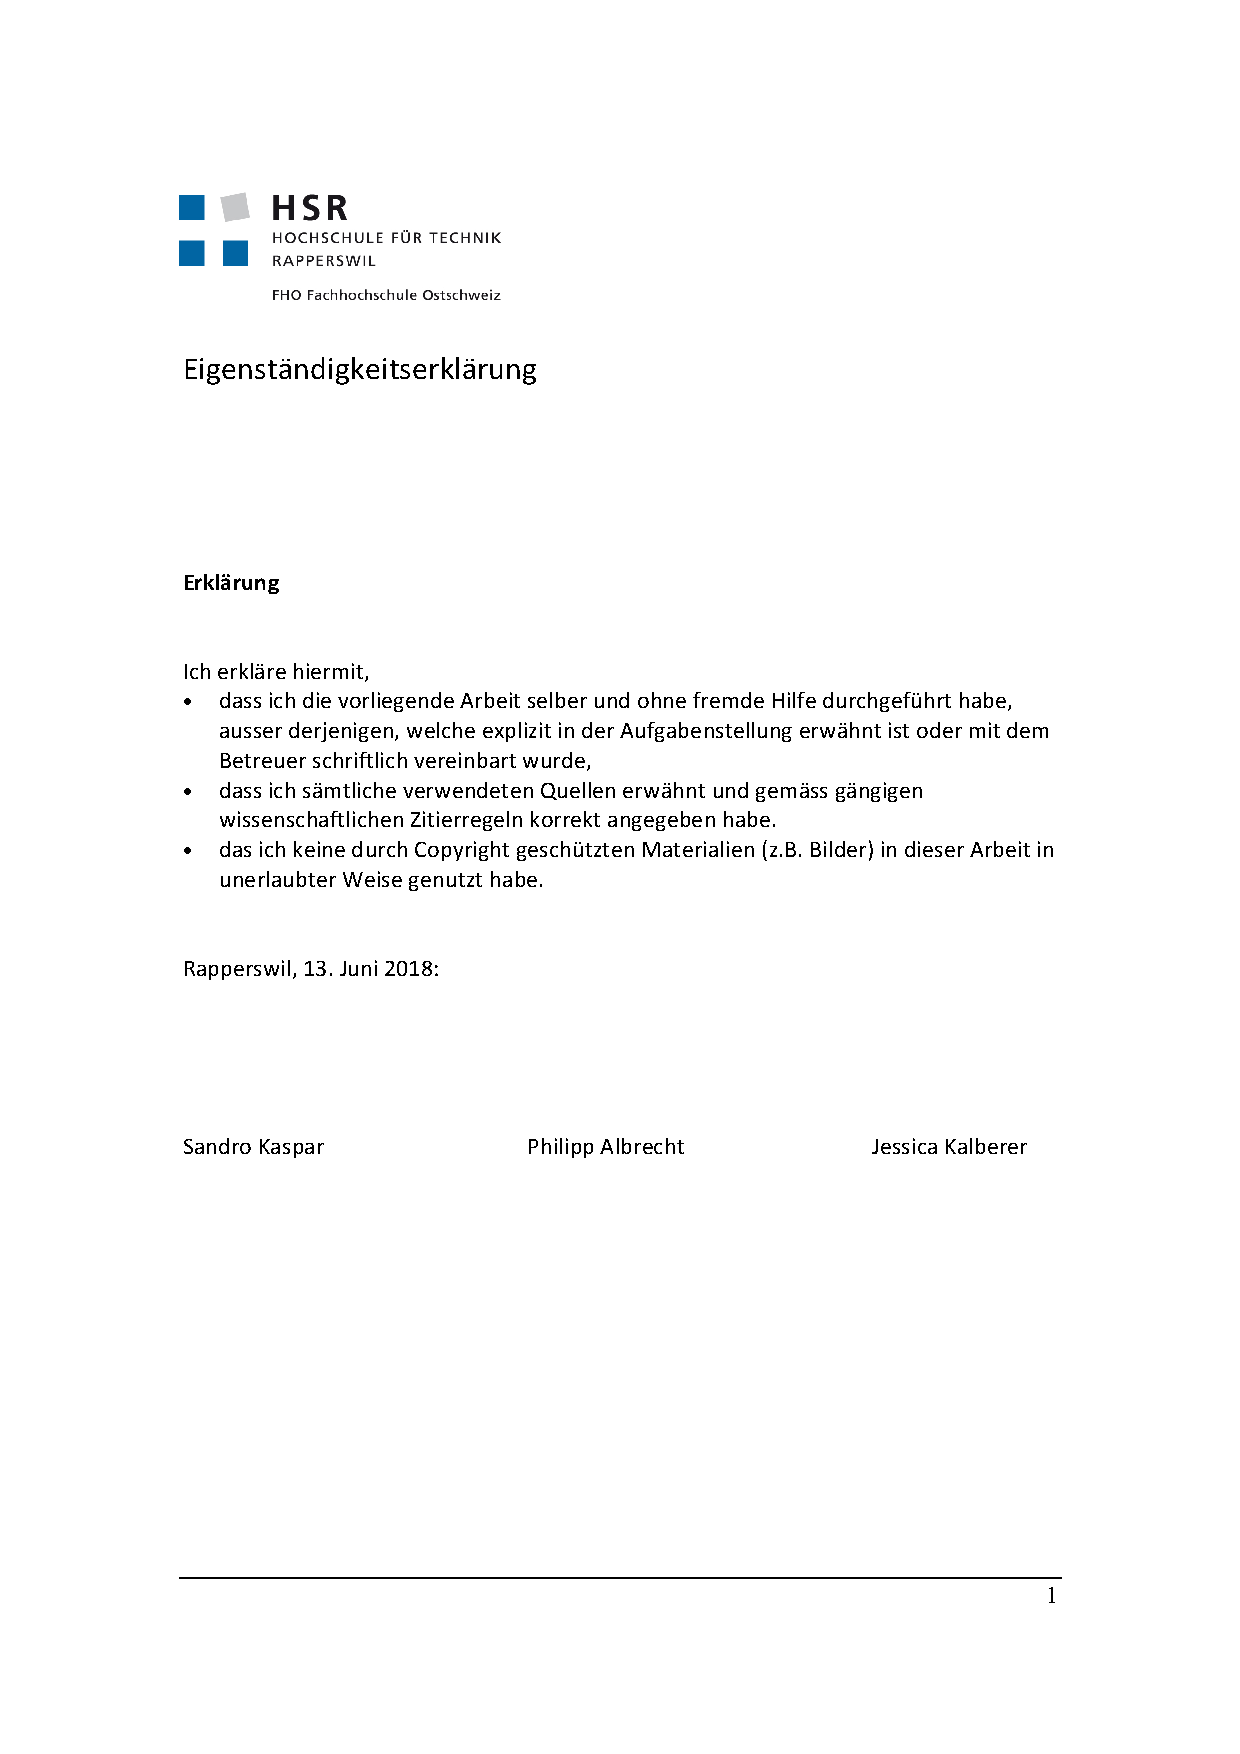
\includepdf[scale=1.0,pages={1}]{pdfincludes/eigenstaendigkeit}
\newpage
\subsection{Urheberrechtsvereinbarung}
%
\includepdf[scale=1.0,pages={1}]{pdfincludes/urheberrecht}


\renewcommand{\listtablename}{Tabellenverzeichnis}
\listoftables
\addcontentsline{toc}{section}{\listtablename}
\renewcommand{\listfigurename}{Abbildungsverzeichnis}
\listoffigures
\addcontentsline{toc}{section}{\listfigurename}
\clearpage
\renewcommand{\refname}{Literaturverzeichnis}
\addcontentsline{toc}{section}{Literaturverzeichnis}
\begin{thebibliography}{}
	\bibitem{rfc-7348} RFC7348 \textit{Virtual eXtensible Local Area Network (VXLAN): A Framework
	for Overlaying Virtualized Layer 2 Networks over Layer 3 Networks}, RFC 7348, 2014 (URL: \url{https://tools.ietf.org/html/rfc7348})
	
	\bibitem{rfc-6830} RFC6830 \textit{The Locator/ID Separation Protocol (LISP)}, RFC 6830, 2014 (URL: \url{https://tools.ietf.org/html/rfc6830})

	\bibitem{sda-whitepaper} SDA White Paper \textit{Software-Defined Access 1.0 Solution White Paper}, 2017 (URL: \url{https://www.cisco.com/c/en/us/solutions/collateral/enterprise-networks/software-defined-access/white-paper-c11-739642.html})
	
	\bibitem{sda-designguide} SDA Design Guide \textit{Software-Defined Access Design Guide}, 2018 (URL: \url{https://www.cisco.com/c/dam/en/us/td/docs/solutions/CVD/Campus/CVD-Software-Defined-Access-Design-Guide-2018JAN.pdf})
	
	\bibitem{sda-definition} SDA Cisco Definition \textit{Software Defined Access Cisco Definition}, 2018 (URL: \url{https://www.cisco.com/c/en/us/solutions/enterprise-networks/software-defined-access/index.html})
	
	\bibitem{campusfabric-introduction} Campus Fabric \textit{Cisco Campus Fabric Introduction}, 2017 (URL: \url{https://www.cisco.com/c/dam/m/hr\_hr/training-events/2017/cisco-connect/pdf/Cisco-Campus-Fabric-Introduction.pdf})
	
	\bibitem{cisco-dna-installation-guide} \textit{Cisco Digital Network Architecture Center Appliance Installation}, 2018 (URL: \url{https://www.cisco.com/c/en/us/td/docs/cloud-systems-management/network-automation-and-management/dna-center/1-1/install/b_dnac_install_1_1_0P2.pdf})

	\bibitem{cisco-dna-installation-guide} \textit{Cisco Digital Network Architecture Center Appliance Installation}, 2018 (URL: \url{https://www.cisco.com/c/en/us/td/docs/cloud-systems-management/network-automation-and-management/dna-center/1-1/install/b_dnac_install_1_1_0P2.pdf})

	\bibitem{cisco-dna-user-guide} \textit{Cisco Digital Network Architecture Center User Guide, Release 1.1}, 2018 (URL: \url{https://www.cisco.com/c/en/us/td/docs/cloud-systems-management/network-automation-and-management/dna-center/1-1/user_guide/b_dnac_ug_1_1.pdf})
	
	\bibitem{cisco-dna-release-notes-1-1-3} \textit{Release Notes for Cisco Digital Network Architecture Center, Release 1.1.3} (URL: \url{https://www.cisco.com/c/en/us/td/docs/cloud-systems-management/network-automation-and-management/dna-center/1-1/rn_release_1_1_3/b_dnac_release_notes_1_1_3.html}), 2018
	
	\bibitem{cisco-pnp-dhcp} \textit{Cisco Open Plug-n-Play Agent Configuration Guide - DHCP Option-based Discovery} (URL: \url{https://www.cisco.com/c/en/us/td/docs/ios-xml/ios/pnp/configuration/xe-3e/pnp-xe-3e-book.html#concept_4A3D8AD59EAE4339B5E7FC7DA73C3594}), 10.05.2018
	
	\bibitem{cisco-dna-appliance-fresh-installation} \textit{Cisco Digital Network Architecture Center Appliance Installation Guide, Release 1.0 - Install a New ISO on the Appliance
	} (URL: \url{https://www.cisco.com/c/en/us/td/docs/cloud-systems-management/network-automation-and-management/dna-center/1-0-x/app_install_guide/b_dnac_install_1_0/b_dnac_install_1_0_chapter_010.html#concept_dxd_tfy_k1b}), 19.05.2018

	\bibitem{cisco-3850-faq} \textit{Cisco Catalyst 3850 Series Switches FAQ} (URL: \url{https://www.cisco.com/c/en/us/products/collateral/switches/catalyst-3850-series-switches/qa_c67-722110.html}), 22.05.2018	

	\bibitem{cisco-dna-appliance-installation-guide-release-1-1} \textit{Cisco Digital Network Architecture Center Appliance Installation Guide, Release 1.1} (URL: \url{https://www.cisco.com/c/en/us/td/docs/cloud-systems-management/network-automation-and-management/dna-center/1-1/install/b_dnac_install_1_1_0P2/b_dnac_install_1_1_0P2_chapter_010.html}), 28.05.2018
	
	\bibitem{infoblox} \textit{Infoblox Information} (URL: \url{https://www.infoblox.com/}), 04.06.2018
	
	\bibitem{infoblox-communityblog} \textit{Infoblox Community Blog about Cisco Integrations} (URL: \url{https://community.infoblox.com/t5/Community-Blog/Infoblox-Cisco-integrations-will-make-you-a-Networking-and/ba-p/12264}), 04.06.2018
	
\end{thebibliography}



\end{document}
